Kiến trúc vi dịch vụ chia dự án thành các thành phần nhỏ hơn được gọi là các dịch vụ.

Các dịch vụ chịu trách nhiệm cho một chức năng cụ thể nhằm hiện thực hóa khả năng kinh doanh cụ thể.

Các dịch vụ độc lập về ngôn ngữ lập trình, CSDL, triển khai,...

Các dịch vụ tương tác với nhau qua hạ tầng mạng.

\begin{figure}[h]

\centering

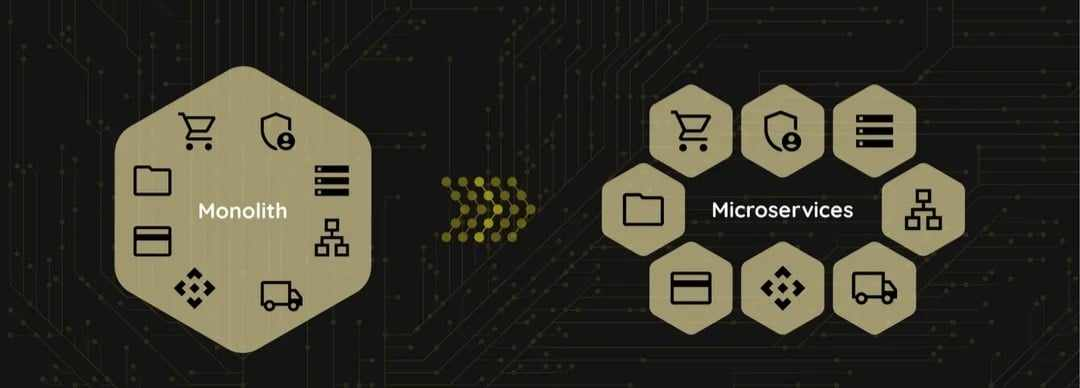
\includegraphics[height = 3cm]{pictures/ChuyenTu_KienTrucNguyenKhoi_Sang_KienTrucViDichVu.jpg}

% \caption{ViDuHinhAnhTheoChieuDoc}

\end{figure}

\begin{figure}[h]

\centering

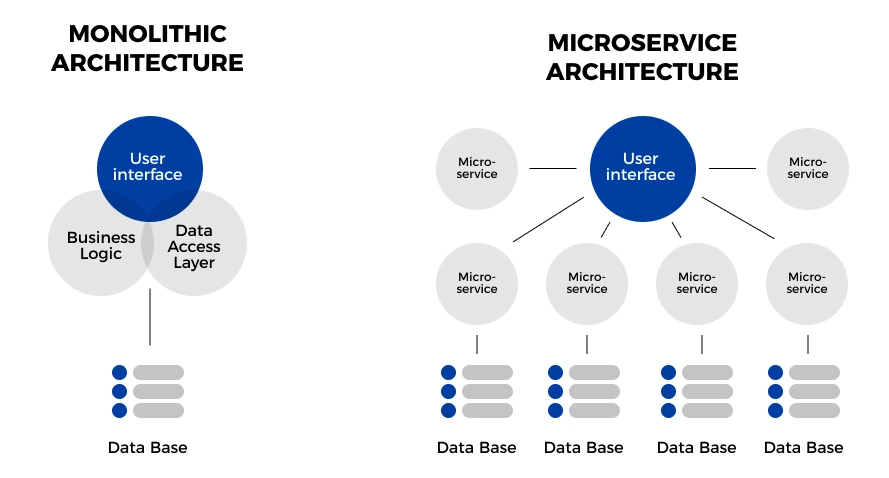
\includegraphics[height = 3cm]{pictures/AnhKhacNhau_KienTrucNguyenKhoi_KienTrucViDichVu.png}

% \caption{ViDuHinhAnhTheoChieuDoc}

\end{figure}

% Strangler Fig là chuyển mono sang dịch vụ

Kiến trúc kiến trúc vi dịch vụ (hay đơn giản là kiến trúc vi dịch vụ) là một cách xây dựng các ứng dụng phần mềm dưới dạng tập hợp các dịch vụ nhỏ, độc lập giao tiếp với nhau thông qua API. Mỗi dịch vụ tập trung vào một khả năng kinh doanh cụ thể và có thể được triển khai, mở rộng quy mô và duy trì độc lập với các dịch vụ khác trong hệ thống. Cách tiếp cận này nhấn mạnh tính mô - đun, tính linh hoạt và khả năng phục hồi, cho phép các nhóm làm việc đồng thời trên các phần khác nhau của hệ thống và cho phép phát hành nhanh hơn và thường xuyên hơn. Các vi dịch vụ thường dựa vào các giao thức truyền thông nhẹ, chẳng hạn như REST và thường được triển khai bằng các công nghệ chứa trong bộ chứa như Docker và Kubernetes.

Đặc trưng

Dưới đây là một số đặc điểm của một kiến trúc kiến trúc vi dịch vụ tốt:

Mô - đun hóa : Kiến trúc nên bao gồm một tập hợp các dịch vụ được kết hợp lỏng lẻo có thể được triển khai, duy trì và mở rộng quy mô một cách độc lập.

Triển khai độc lập : Mỗi dịch vụ phải có khả năng triển khai độc lập để có thể thực hiện các thay đổi đối với một dịch vụ mà không ảnh hưởng đến các dịch vụ khác.

Bối cảnh giới hạn : Kiến trúc phải được thiết kế để phù hợp với ranh giới của khả năng kinh doanh, sao cho mỗi dịch vụ chịu trách nhiệm về một tập hợp chức năng cụ thể, gắn kết.

Tự chủ : Các dịch vụ phải có khả năng hoạt động tự chủ, ít phụ thuộc vào các dịch vụ khác.

Khả năng phục hồi : Kiến trúc phải được thiết kế để chịu đựng lỗi và các dịch vụ phải có khả năng xử lý lỗi một cách duyên dáng.

Khả năng mở rộng : Kiến trúc phải được thiết kế để hỗ trợ mở rộng quy mô các dịch vụ riêng lẻ cũng như toàn bộ hệ thống.

Tính linh hoạt : Kiến trúc phải cho phép phát triển và triển khai nhanh chóng các dịch vụ mới cũng như khả năng thay đổi các dịch vụ hiện có một cách nhanh chóng và dễ dàng.

Văn hóa DevOps : Kiến trúc phải được hỗ trợ bởi văn hóa nhấn mạnh sự cộng tác và giao tiếp giữa các nhóm phát triển và vận hành, cũng như tự động hóa các quy trình triển khai và thử nghiệm.

Nhược điểm

Mặc dù kiến trúc vi dịch vụ có nhiều lợi ích nhưng cũng có một số nhược điểm cần xem xét:

Độ phức tạp ngày càng tăng : Kiến trúc kiến trúc vi dịch vụ phức tạp hơn kiến trúc nguyên khối. Bản chất phân tán của kiến trúc vi dịch vụ khiến việc phát triển, thử nghiệm, triển khai và giám sát hệ thống trở nên khó khăn hơn.

Những thách thức về điện toán phân tán : Với kiến trúc vi dịch vụ, các dịch vụ khác nhau có thể chạy trên các máy khác nhau, khiến việc duy trì liên lạc giữa chúng trở nên khó khăn. Điều này có thể dẫn đến các vấn đề về độ trễ, tính nhất quán của dữ liệu và độ tin cậy.

Chi phí hoạt động : Với kiến trúc kiến trúc vi dịch vụ, có nhiều dịch vụ cần triển khai và quản lý, điều này có thể dẫn đến tăng chi phí hoạt động.

Ranh giới dịch vụ : Việc xác định ranh giới dịch vụ có thể là một thách thức, đặc biệt là trong các hệ thống phức tạp. Nếu không được thiết kế chính xác, điều này có thể dẫn đến sự phụ thuộc vào dịch vụ khiến việc thay đổi một dịch vụ trở nên khó khăn hơn.

Thách thức về tích hợp : kiến trúc vi dịch vụ thường yêu cầu tích hợp với các dịch vụ khác, điều này có thể khó đạt được. Các dịch vụ có thể có các giao thức, định dạng dữ liệu và phương thức liên lạc khác nhau, điều này có thể gây khó khăn cho việc tích hợp.

Chi phí chung của cổng API : Cần có cổng API để quản lý các API dịch vụ khác nhau và cung cấp giao diện hợp nhất cho khách hàng. Điều này có thể bổ sung thêm chi phí cho hệ thống.

Gỡ lỗi và kiểm tra: Việc gỡ lỗi và kiểm tra có thể phức tạp hơn trong kiến trúc kiến trúc vi dịch vụ do tính chất phân tán của hệ thống.

Nhìn chung, những nhược điểm của kiến trúc kiến trúc vi dịch vụ có thể được giảm thiểu bằng các phương pháp thiết kế và phát triển tốt. Tuy nhiên, điều quan trọng là phải cân nhắc giữa lợi ích và nhược điểm khi quyết định có nên sử dụng kiến trúc kiến trúc vi dịch vụ hay không.
